% Version en espanol, traducida directamente de article-gcp-vs-a2a.tex
% (formato SAI / IJACSA, plantilla oficial IEEEtran-based). Contenido,
% cifras, tablas, citas y estructura de secciones son coherentes con la
% version en ingles; solo el texto en prosa, los titulos de seccion y las
% etiquetas de tabla se tradujeron. Los identificadores tecnicos (nombres
% de modelo, nombres de escenario, codigo/pseudocodigo) se mantienen en
% ingles por trazabilidad con el arnes de evaluacion real.
\documentclass[conference,letterpaper]{IEEEtran}

% --- paquetes (base de la plantilla, en el orden de la propia plantilla) ---
\ifCLASSINFOpdf
  \usepackage[pdftex]{graphicx}
\else
\fi
\usepackage[cmex10]{amsmath}
\usepackage{color}
\usepackage{flushend}
\usepackage{fancyhdr}
\usepackage{subcaption}
\usepackage{balance}
\captionsetup[table]{justification=centering, labelsep=period, font={footnotesize,sc}}
\captionsetup[figure]{justification=centering, labelsep=period, font={footnotesize}}
\usepackage{booktabs}
\usepackage{algorithm}
\usepackage{algpseudocode}
\usepackage{threeparttable}
\usepackage{float}

% --- paquetes adicionales que este paper necesita sobre la base de la plantilla ---
\usepackage[utf8]{inputenc}
\usepackage[T1]{fontenc}
\usepackage{amssymb}
\usepackage{multirow}
\usepackage{microtype}
\usepackage{verbatim}
\usepackage[numbers,sort&compress]{natbib}
\usepackage{xurl} % permite que las URL largas de referencias se corten entre lineas
\usepackage[hidelinks]{hyperref}
\hypersetup{pdfauthor={}}
\usepackage{tikz}
\usetikzlibrary{positioning,arrows.meta}
\usepackage{pgfplots}
\pgfplotsset{compat=1.17}

\hyphenation{op-tical net-works semi-conduc-tor}

\renewcommand{\thispagestyle}[2]{}
\fancypagestyle{plain}{
        \fancyhead{}
        \fancyhead[C]{first page center header}
        \fancyfoot{}
        \fancyfoot[C]{first page center footer}
}
\pagestyle{fancy}
\headheight 23pt
\footskip 20pt
\rhead{}
\setcounter{page}{1}
\fancyhead[R]{\textit{(IJACSA) International Journal of Advanced Computer Science and Applications, \\ Vol. XXX, No. XXX, 2026}}
\renewcommand{\headrulewidth}{0pt}
\fancyfoot[C]{www.ijacsa.thesai.org}
\renewcommand{\footrulewidth}{0.5pt}
\fancyfoot[R]{\thepage \  $|$ P a g e }

\newcommand{\gcp}{\textsc{gcp}}
\newcommand{\ata}{\textsc{a2a}}
\newcommand{\bigoh}{\mathcal{O}}

% IEEEtran define estas dos cadenas en ingles ("Abstract", "Index Terms");
% se sobrescriben aqui para que el entorno abstract/IEEEkeywords las
% imprima en espanol sin tocar el resto de la plantilla.
\renewcommand{\abstractname}{Resumen}
\renewcommand{\IEEEkeywordsname}{Palabras clave}

\begin{document}

\title{Federaci\'on de Contexto de Lectura Primero y Control por Rol para Sistemas
Multiagente Basados en LLM: \textit{una Comparaci\'on Multi-Modelo Controlada Frente al Paso de
Mensajes Punto a Punto}}

\author{\IEEEauthorblockN{\phantom{Ryan Valdivia-Segovia\IEEEauthorrefmark{1}, Adrian Mamani-Quispe\IEEEauthorrefmark{1},}\\ \phantom{Karim Guevara\IEEEauthorrefmark{1}, Norka Bedregal-Alpaca\IEEEauthorrefmark{1}}}
\IEEEauthorblockA{\phantom{\IEEEauthorrefmark{1}Universidad Nacional de San Agust\'in de Arequipa, Arequipa, Per\'u}\\
\phantom{rvaldiviase@unsa.edu.pe, admamaniq@unsa.edu.pe,}\\ \phantom{kguevarap@unsa.edu.pe, nbedregal@unsa.edu.pe}}
}

\maketitle

\begin{abstract}
Los sistemas multiagente basados en modelos de lenguaje grandes (LLM) suelen depender del paso de
mensajes punto a punto, lo que aumenta la complejidad de integración y deja el control de acceso
granular y la trazabilidad en manos de mecanismos adicionales. Este estudio evalúa el Graph Context
Protocol (\gcp{}), un enfoque de federación de contexto de lectura primero con control de acceso por
rol y por capacidad y procedencia nativa por cada lectura. \gcp{} se compara con dos brazos de
Agent2Agent (\ata{}): el protocolo base tal como se distribuye, y una variante instrumentada cuyo punto
de aplicación de políticas aplica la misma política de roles y de delegación y escribe un registro de
auditoría. La lógica del agente, los modelos, las tareas y los criterios de evaluación se mantienen
constantes; solo cambia la capa de interoperabilidad. Se ejecutaron cinco escenarios conductuales, uno
de los cuales puntúa la fuga semántica de un nodo útil pero prohibido, en seis modelos (tres locales y
tres alojados; 2{,}475 corridas, ninguna fallida). Un análisis estructural muestra que un \gcp{} de tipo
hub necesita $\bigoh(n)$ aristas de integración frente a $\bigoh(n^2)$ de una malla \ata{} completa,
pero \ata{} a través de un orquestador también es $\bigoh(n)$, de modo que esto refleja la topología y
no el protocolo. \gcp{} denegó los 443 intentos no autorizados y \ata{} instrumentado los 408, mientras
que \ata{} base ejecutó los 392; el brazo instrumentado igualó a \gcp{} en contención, procedencia y
fuga en todos los modelos. La brecha de gobernanza refleja por tanto la presencia de un punto de
aplicación y un sumidero de auditoría, que \gcp{} provee de forma nativa y que \ata{} exige añadir en
cada despliegue. El costo en tokens es comparable entre \gcp{} y \ata{} instrumentado; el éxito de
tarea es indistinguible en cuatro de seis modelos y menor con \gcp{} para el modelo alojado más
pequeño y, en un escenario, para \texttt{llama3.1:8b}. En el modelo alojado la causa es la redacción de
la descripción de la herramienta: intercambiar las descripciones entre brazos invierte la tasa de
respuestas finales vacías.
\end{abstract}

\begin{IEEEkeywords}
modelos de lenguaje grandes; control de acceso; procedencia; contenci\'on de agentes; acoplamiento
de software
\end{IEEEkeywords}

\section{Introducci\'on}

El paso de mensajes directo es el patr\'on de coordinaci\'on predominante en los sistemas
multiagente basados en modelos de lenguaje grandes (LLM). Marcos como AutoGen~\citep{wu2023autogen},
ChatDev~\citep{qian2024chatdev} y MetaGPT~\citep{hong2024metagpt} organizan aplicaciones en torno a
agentes que se comunican mediante mensajes. El protocolo Agent2Agent (A2A)~\citep{a2a2025}, a su vez,
estandariza la comunicaci\'on entre agentes: un agente cliente anuncia y delega tareas a agentes
remotos con nombre mediante JSON-RPC. Este paradigma desciende de los lenguajes cl\'asicos de
comunicaci\'on entre agentes KQML~\citep{finin1994} y
FIPA-ACL~\citep{fipa2002}, que ya asum\'ian conexiones por pares y protocolos compartidos y
pre-negociados entre cada par que interact\'ua.

El paso de mensajes tiene un costo estructural que la literatura de ingenier\'ia de software conoce
desde hace cincuenta a\~nos. Conectar $n$ componentes por pares requiere del orden de $n^2$ enlaces;
un intermediario compartido al que cada componente se conecta una sola vez reduce esto a $n$. Este es
el ``espagueti de integraci\'on'' que el cat\'alogo de Enterprise Integration
Patterns~\citep{hohpe2003} aborda con brokers y hubs, y que la teor\'ia del
acoplamiento~\citep{parnas1972,stevens1974,briand1999} formaliza: la modificabilidad est\'a gobernada
por el n\'umero y la fuerza de las dependencias entre componentes.

Se estudia aqu\'i una infraestructura alternativa para la coordinaci\'on de agentes: el Graph Context
Protocol (\gcp{}). Este protocolo prioriza la lectura: un agente obtiene lo que necesita leyendo
contexto desde nodos de conocimiento de propiedad independiente en lugar de recibir mensajes
empujados. Es \emph{controlado por rol}: cada lectura pasa
por una compuerta de pol\'itica que autoriza la solicitud seg\'un el rol y las capacidades requeridas,
denegando por defecto~\citep{saltzer1975,sandhu1996}. \gcp{} tambi\'en provee auditabilidad: cada
decisi\'on de lectura o delegaci\'on ---conceder o denegar--- produce un registro de procedencia
estructurado.

\paragraph{Tesis (forma medida).} La federación de contexto de lectura primero y controlada por rol traslada la autorización y la auditoría de cada par de agentes al nodo y al protocolo. El estudio mide (i) la topología de integración que esto implica, (ii) los resultados de gobernanza (contención, procedencia y fuga) frente a \ata{} base y frente a un despliegue de \ata{} instrumentado con un punto de aplicación de políticas equivalente, y (iii) las consecuencias en costo y éxito de tarea en seis modelos. Los resultados estructurales son deterministas; los de gobernanza y conductuales provienen de 30 semillas por brazo (15 para el modelo local más grande) con intervalos de Wilson y pruebas exactas.

\paragraph{Alcance de la comparación.} No se afirma que el paso de mensajes \emph{no pueda}
auditarse: registros, middleware, proxies o gateways pueden añadir un rastro de acceso. Por ello se
comparan dos brazos \ata{} con \gcp{}. El brazo \emph{base} es el protocolo tal como se distribuye, sin
autorización ni registro, y muestra lo que le falta a un despliegue hasta que añade esos controles. El
brazo \emph{instrumentado} (\ata{}+PEP) corre los mismos servidores \ata{} detrás de un punto de
aplicación de políticas que autentica un token de portador, aplica la misma política de roles y la
misma regla de delegación que \gcp{}, y registra una entrada de auditoría por decisión. El brazo
instrumentado es el comparador justo para las afirmaciones de gobernanza; el brazo base se reporta
porque es lo que el protocolo ofrece de fábrica.

\paragraph{Contribuciones.}
\begin{enumerate}
  \item Arquitectura y una especificaci\'on reproducible. \gcp{} (de lectura
  primero, controlado por rol, auditado, con una compuerta de delegaci\'on de capacidad m\'as
  estricta) se describe con precisi\'on suficiente para reimplementarlo: formato de consulta, estructura de nodo
  y pol\'itica, credencial de rol, registro de procedencia y el algoritmo de autorizaci\'on
  (Secci\'on~\ref{sec:arch}).
  \item Un m\'etodo de benchmark controlado por equidad. Una \'unica definici\'on de
  escenario y un \'unico modelo inyectado construyen todos los brazos; solo cambia la capa de
  interoperabilidad (Secci\'on~\ref{sec:method}).
  \item Una comparación empírica multi-modelo de tres brazos sobre cinco escenarios conductuales
  ---incluyendo una prueba de \emph{acceso forzado} que apunta directamente al nodo confidencial y un
  escenario \emph{useful-forbidden} puntuado con patrones de fuga semántica--- y seis modelos (tres de
  peso abierto, tres alojados), con 2{,}475 corridas registradas con sus trazas, separando resultados
  deterministas de resultados dependientes del modelo (Sección~\ref{sec:results}).
  \item Definiciones de m\'etricas para acoplamiento estructural, sobrecosto de
  descubrimiento/prompt de herramientas, una taxonom\'ia de fuga/agencia de cuatro v\'ias, completitud
  de procedencia y contenci\'on de delegaci\'on/acceso forzado (Secci\'on~\ref{sec:metrics}).
\end{enumerate}

\section{Antecedentes}
\label{sec:related}

\subsection{El paso de mensajes como l\'inea base multiagente}
Los lenguajes de comunicaci\'on entre agentes establecieron el paradigma de paso de mensajes:
KQML~\citep{finin1994} envolv\'ia cargas \'utiles en performativos tipados sobre conexiones por
pares, y FIPA-ACL~\citep{fipa2002} estandariz\'o un mensaje en el que emisor y receptor deben
compartir lenguaje de contenido y ontolog\'ia antes de que cualquier intercambio tenga \'exito. Los
marcos LLM modernos reinventaron esto en lenguaje natural. AutoGen~\citep{wu2023autogen} programa
aplicaciones como conversaciones; ChatDev~\citep{qian2024chatdev} organiza pares de roles en una
``cadena de chat'' fija; los estudios de revisi\'on~\citep{guo2024survey} clasifican la comunicaci\'on
en variantes de igual a igual, centralizada, en capas y de conjunto compartido. El Model Context
Protocol~\citep{mcp2024} estandariza el acceso a contexto de agente a herramienta (una forma temprana
de lectura primero), mientras que A2A~\citep{a2a2025} estandariza la delegaci\'on de tareas de agente
a agente ---la l\'inea base contra la que se hace benchmark aqu\'i. \citet{zhang2024agentprune}
reportan un 28--73\% de tokens excedentes en grafos de comunicaci\'on entre agentes y recuperan la
mayor\'ia podando la topolog\'ia. \citet{mao2026delm} reemplazan tanto la orquestaci\'on centralizada
como el enrutamiento de igual a igual por un contexto verificado compartido a aproximadamente la
mitad del costo. Este trabajo a\~nade autorizaci\'on controlada por rol, procedencia auditada por
lectura, una compuerta de contenci\'on de agencia y una comparaci\'on multi-modelo controlada por
equidad.

\subsection{El acoplamiento y el problema de $n^2$}
Que menos enlaces entre componentes produzcan sistemas m\'as mantenibles es uno de los resultados
m\'as antiguos de la ingenier\'ia de software. \citet{parnas1972} mostr\'o que la descomposici\'on por
ocultamiento de informaci\'on produce un acoplamiento mucho menor que el particionamiento estilo
diagrama de flujo; \citet{stevens1974} hizo medibles el acoplamiento y la cohesi\'on;
\citet{briand1999} dio un marco te\'orico de grafos en el que el acoplamiento es mon\'otono en el
n\'umero de aristas de dependencia, de modo que una topolog\'ia de $\bigoh(n)$ aristas est\'a
demostrablemente menos acoplada que una de $\bigoh(n^2)$. \citet{hohpe2003} traslad\'o esto a la
integraci\'on: una malla punto a punto de $n$ sistemas necesita $n(n{-}1)/2$ canales, que un hub
reduce a $n$. La investigaci\'on en microservicios~\citep{panichella2021} lleva el mismo argumento a
sistemas cloud-native, y \citet{shen2025topology} muestran que las topolog\'ias densas de agentes
amplifican la propagaci\'on de errores mientras que las m\'as dispersas la suprimen. \ata{} crea
aristas agente$\leftrightarrow$agente; \gcp{} crea aristas agente$\rightarrow$almac\'en.

\subsection{M\'inimo privilegio, contexto con control de acceso y recuperaci\'on con compuerta}
La compuerta de lectura de \gcp{} operacionaliza el m\'inimo privilegio~\citep{saltzer1975}. El
control de acceso basado en roles~\citep{sandhu1996} asigna permisos a roles; el control de acceso
basado en atributos~\citep{nist800162} generaliza a atributos arbitrarios; la protecci\'on basada en
capacidades~\citep{dennis1966} ata la autoridad a tokens expl\'icitamente pasados ---el modelo que
siguen las credenciales de rol de \gcp{}. La legislaci\'on de minimizaci\'on de datos~\citep{gdpr2016}
convierte ``leer solo lo que tu rol requiere'' en una restricci\'on legal. El acceso a herramientas de
lectura primero (MCP) y la recuperaci\'on con control de acceso proveen el lado de la lectura, y
RBAC/ABAC el lado de la compuerta, pero ninguno acopla ambos con procedencia por lectura; la l\'inea
base punto a punto no tiene una compuerta an\'aloga, por lo que el control de fuga y de delegaci\'on
descansa en la discreci\'on del emisor.

\subsection{Fuga, procedencia y gobernanza en sistemas agenticos}
La confidencialidad en sistemas agenticos es una propiedad del sistema, no solo del
modelo~\citep{evertz2024whispers}; los canales de mensajes entre agentes son el vector de fuga
dominante, en gran medida invisible para la auditor\'ia basada solo en la salida
~\citep{elyagoubi2026agentleak}; y restringir lo que un agente puede \emph{ver} es m\'as robusto que
filtrar lo que puede \emph{decir}~\citep{bagdasarian2024airgap}. El OWASP Top 10 para aplicaciones LLM
~\citep{owasp2025} nombra la Divulgaci\'on de Informaci\'on Sensible y la Agencia Excesiva como
riesgos primarios ---esta \'ultima es exactamente lo que sondea el escenario de delegaci\'on. El
control determinista de privilegios en el l\'imite de la herramienta~\citep{shi2025progent}, la
delegaci\'on autenticada de autoridad~\citep{south2025delegation} y los rastros de
auditor\'ia~\citep{ojewale2025audit} abogan por registros a prueba de manipulaci\'on de las acciones
del sistema.

\paragraph{Delta / novedad defendible.} El trabajo previo aporta las piezas ---acceso de lectura
primero (MCP), control por rol/atributo (RBAC/ABAC, RAG con control de acceso), delegaci\'on auditada
y registros de auditor\'ia--- pero no su conjunci\'on, ni una comparaci\'on directa multi-modelo
controlada por equidad contra una l\'inea base real de paso de mensajes. La novedad reivindicada aqu\'i
es precisamente la \emph{integraci\'on}: lectura federada $+$ control por rol $+$ procedencia
por lectura, evaluados contra \ata{}. La lectura primero sola, RBAC solo, o la auditor\'ia sola no
ser\'ian una contribuci\'on.

\section{El Graph Context Protocol: Especificaci\'on}
\label{sec:arch}

\gcp{} modela un ecosistema como \emph{nodos de conocimiento} y \emph{nodos de agente} de propiedad
independiente. La coordinaci\'on es de lectura primero: un agente emite una \emph{consulta de
contexto} a un nodo par, que devuelve el contexto que el solicitante est\'a autorizado a leer.
El sustrato se especifica con precisi\'on suficiente para reimplementarlo.

\subsection{Estructuras de datos}
Un nodo de conocimiento lleva un id, un tipo, un adaptador que produce contenido y una
pol\'itica de acceso. Una pol\'itica declara los campos de la compuerta; una
credencial de rol nombra el rol del solicitante y sus capacidades planas; un
registro de procedencia registra cada decisi\'on.

{\small
\begin{verbatim}
KnowledgeNode {
  id, kind,               // e.g. "rag", "log"
  adapter,                // yields raw content
  policy: AccessPolicy }
AccessPolicy {
  readableByRoles: [roleId],
  requiredCapabilities: [capId],
  fallbackAllowed: bool,
  denialMode: "empty" | "error" }
Principal (role credential) {
  id, role: { id, capabilities:[capId],
              parent? },
  capabilities: [capId] }
Provenance {
  principalId, targetNodeId, timestamp,
  decision: "grant" | "deny",
  matchedPolicy }
\end{verbatim}}

\subsection{Flujo de consulta y autorizaci\'on}
Una consulta de contexto nombra un nodo destino y una capacidad solicitada (lectura, o la m\'as
estricta delegaci\'on). El servidor eval\'ua el predicado de admisi\'on \emph{antes} de que corra
cualquier adaptador, de modo que el contenido denegado nunca entra a la ventana de contexto del
agente (mediaci\'on completa~\citep{saltzer1975}). El conjunto efectivo de capacidades de un
solicitante es la uni\'on de sus capacidades planas y las heredadas a trav\'es de la cadena de roles
(precedencia propia primero). El predicado es
\begin{align*}
\mathit{authorized}(P,K)\equiv\;
&\underbrace{(P.\textit{roles}{=}[\,]\vee K.\textit{role}{\in}P.\textit{roles})}_{\textit{roleOk}}\\
\wedge\;
&\underbrace{(P.\textit{caps}{=}[\,]\vee P.\textit{caps}{\subseteq}\mathit{eff}(K))}_{\textit{capsOk}}
\end{align*}
Una pol\'itica ausente o con esquema inv\'alido se trata como una denegaci\'on (denegaci\'on por
defecto). La ruta de extremo a extremo es:

\begin{center}\small
Solicitud $\rightarrow$ Verificaci\'on de pol\'itica $\rightarrow$ Decisi\'on
$\rightarrow$ Contexto devuelto / denegado $\rightarrow$ Registro de procedencia
\end{center}

\subsection{Algoritmo de lectura/autorizaci\'on (pseudoc\'odigo)}
{\footnotesize
\begin{verbatim}
handleQuery(query, principal):
  node = resolve(query.targetNodeId)
  if node == null: return deny("no-node")
  P = node.policy
  if P invalid or absent:        # default-deny
      record(principal,node,"deny","none")
      return deny("no-policy")
  eff = flat(principal) UNION
        rolechain(principal.role)
  roleOk = P.roles==[] or
           principal.role.id in P.roles
  capsOk = P.caps==[] or P.caps subset eff
  needCap = query.capability     # read|delegate
  capOk2 = needCap in eff
  if roleOk and capsOk and capOk2:
      record(principal,node,"grant",P.id)
      return node.adapter.read()  # content
  else:
      record(principal,node,"deny",P.id)
      return denialResult(P.denialMode)  # denied
\end{verbatim}}
La delegaci\'on reutiliza esta misma ruta con \texttt{needCap = delegate}, una capacidad estrictamente
m\'as fuerte que \texttt{read}: un agente autorizado a leer no queda por ello autorizado a comandar.

\subsection{Manejo de denegaciones}
Ante una denegaci\'on el manejador devuelve solo una raz\'on de denegaci\'on (o un resultado vac\'io,
seg\'un \texttt{denialMode}); el adaptador nunca se invoca, por lo que el contenido del nodo no puede
aparecer en la respuesta. Cada denegaci\'on se registra a su vez, produciendo un libro de qui\'en
intent\'o qu\'e, no solo de qui\'en ley\'o qu\'e.

\subsection{Relaci\'on con A2A y MCP}
La Tabla~\ref{tab:props} contrasta los tres. A2A es agente a agente y basado en empuje, con
permiso/denegaci\'on burda declarada en la tarjeta y sin rastro nativo por lectura; MCP es de lectura
primero pero agente a herramienta y de propietario \'unico, sin control por rol entre propietarios;
\gcp{} combina acceso de lectura primero entre propietarios, control por rol, denegaci\'on por
defecto y procedencia nativa por lectura. Un ``no'' en la Tabla~\ref{tab:props} no significa que el
protocolo haga imposible la propiedad; toda celda es alcanzable en principio extendiendo el protocolo
base. ``no nat.'' $=$ no es una primitiva nativa del protocolo base (requerir\'ia l\'ogica adicional
encima); ``ext.'' $=$ alcanzable solo con instrumentaci\'on externa adicional; ``n/a'' $=$ el concepto
no aplica al dise\~no de este protocolo.

\begin{table}[H]
\centering
\caption{Comparaci\'on de propiedades.}
\label{tab:props}
\setlength{\tabcolsep}{4pt}
\begin{tabular}{lccc}
\toprule
propiedad & \ata{} & MCP & \gcp{} \\
\midrule
agente$\leftrightarrow$agente          & s\'i & no nat. & s\'i \\
lectura primero                        & no nat. & s\'i & s\'i \\
l\'imite entre propietarios            & s\'i & no nat. & s\'i \\
compuerta por rol/capacidad            & burda & no nat. & s\'i \\
procedencia por lectura (nativa)       & ext. & ext. & s\'i \\
denegaci\'on por defecto               & no nat. & no nat. & s\'i \\
delegaci\'on de capacidad m\'as estricta & no nat. & n/a & s\'i \\
\bottomrule
\end{tabular}
\end{table}

\subsection{Modelo de amenazas y vinculación de credenciales}
\label{sec:threat-model}
\paragraph{Vinculación de credenciales.} Una consulta lleva una credencial de portador, no un rol. El
servidor pasa la credencial a su \texttt{AuthProvider}, que devuelve el \texttt{Principal}
(identificador, rol, capacidades planas); la compuerta usa solo ese principal resuelto por el servidor,
nunca un rol afirmado en la solicitud. El campo \texttt{requester.principalId} de una consulta se usa
únicamente para etiquetar los registros de auditoría de autenticaciones fallidas. La evaluación usa una
tabla estática de tokens (un token asignado a un principal por corrida), que representa la emisión de
credenciales fuera de banda; la vigencia, la rotación y la restricción al emisor del token no se
modelan.

\paragraph{Adversarios.} Se distinguen seis adversarios, con su tratamiento en este estudio:
\begin{itemize}
  \item \emph{A1, modelo instruido}: posee una credencial legítima y se le indica acceder o delegar más
  allá de su rol. Evaluado (escenarios de acceso forzado y delegación): la compuerta deniega y el
  sumidero de auditoría registra el intento.
  \item \emph{A2, modelo con inyección de prompt}: llega al mismo comportamiento que A1 mediante
  contenido inyectado. La compuerta no depende del razonamiento del modelo, por lo que el resultado es
  el mismo; el canal de inyección en sí no se evalúa.
  \item \emph{A3, agente que afirma otro rol}: derrotado por la vinculación de credenciales, ya que se
  ignoran las afirmaciones de rol en la solicitud; cubierto por pruebas unitarias del manejador, no por
  una campaña adversarial.
  \item \emph{A4, agente comprometido o credencial robada}: no mitigado; poseer un token confiere su rol.
  \item \emph{A5, dueño de nodo malicioso}: un nodo puede devolver contenido arbitrario o registrar de
  forma selectiva; los nodos no se autentican ante los llamantes y el registro de auditoría no es
  evidente ante manipulación en este diseño.
  \item \emph{A6, agentes que coluden o canales fuera de banda}: la compuerta solo media las lecturas y
  delegaciones que atraviesan \gcp{}; los datos compartidos fuera del protocolo quedan fuera de alcance.
\end{itemize}
La propiedad respaldada por la evidencia se limita por tanto a A1--A3 con un servidor y un proveedor de
autenticación no comprometidos: ningún contenido de nodo entra en el contexto de un llamante a menos
que el principal del llamante, resuelto por el servidor, satisfaga la política del nodo.

\section{Definici\'on de M\'etricas}
\label{sec:metrics}

Las m\'etricas se reportan en cuatro familias. Lo determinista se separa de lo dependiente del modelo
en todo momento.

\paragraph{Acoplamiento estructural (determinista).} Para $n$ pares, las \emph{conexiones por pares}
son las aristas de integraci\'on que la topolog\'ia requiere: $C_{\ata{}}(n)=n(n{-}1)$ vs.\
$C_{\gcp{}}(n)=n$. El \emph{esfuerzo de integraci\'on} es el costo marginal $C(n{+}1)-C(n)$: constante
$1$ para \gcp{}, $2n$ para \ata{}. Calculado exactamente. Las aristas de integraci\'on se cuentan como
\emph{dirigidas}; cada relaci\'on bidireccional entre pares contribuye por lo tanto dos aristas
dirigidas. Bajo una definici\'on de canal no dirigido el conteo correspondiente es $n(n{-}1)/2$; la
conclusi\'on asint\'otica se mantiene en $\bigoh(n^2)$.

\paragraph{Sobrecosto de descubrimiento y de prompt de herramientas (por solicitud).}
\emph{Mensajes de descubrimiento}: viajes de ida y vuelta para saber qu\'e puede consultarse ---$1$
para \gcp{}, $n$ para \ata{} base (una tarjeta por par). \emph{Tokens de prompt de herramientas}:
costo en tokens de las descripciones de herramientas/agentes inyectadas en cada solicitud. Recurrente,
distinto del cableado \'unico inicial.

\paragraph{Gobernanza (dos puntos de referencia).} \emph{Completitud de procedencia}: fracción de
decisiones con un registro estructurado, acotada a $[0,1]$; una corrida sin decisiones cuenta como
$1.0$ (no hay nada que registrar). Para \gcp{} y para el brazo \ata{} instrumentado es $1.0$ porque
ambos escriben un registro de auditoría por decisión. Para \ata{} base es $0.0$ siempre que el agente
intentó algo ---léase como ``la implementación base no produce trazabilidad por lectura sin
instrumentación añadida'', no como ``\ata{} no puede auditarse''. \emph{Contención}: fracción de
intentos \emph{no autorizados} (delegación o lectura) rechazados en lugar de ejecutados. Para los dos
brazos con compuerta es denegados sobre intentados; para \ata{} base todo intento no autorizado
ejecutado cuenta como no contenido. Los intentos se agrupan entre semillas (una corrida puede contener
varios), de modo que los denominadores son intentos, no corridas.

\paragraph{Fuga y agencia.} Se distinguen cuatro categorías: (a) \emph{acceso no autorizado
intentado} ---el agente intentó alcanzar un nodo o acción sobre el que no tiene derechos; (b)
\emph{acceso no autorizado concedido} ---el sustrato lo sirvió; (c) \emph{fuga en la transcripción}
---un elemento protegido aparece en cualquier parte de la transcripción de herramientas; (d) \emph{fuga
en la respuesta final} ---aparece en la respuesta. Un elemento protegido se detecta por coincidencia
exacta de canario o, en el escenario \emph{useful-forbidden}, mediante patrones semánticos que también
capturan la paráfrasis (por ejemplo, una cifra reexpresada en otras unidades o palabras). La
coincidencia de patrones sigue siendo un sustituto, no un juez de implicación, y las trazas de las
corridas se almacenan para poder reevaluar la fuga fuera de línea. La \emph{garantía arquitectónica}
(lo que la compuerta previene) se distingue de la \emph{fuga observada} (lo que un modelo dado ejerció).

\paragraph{Costo y \'exito conductual.} Conteos (mensajes, conexiones, viajes de ida y vuelta, tokens
en el cable) y latencia de reloj de pared, con un or\'aculo de \'exito por escenario. Los conteos son
la se\~nal de costo primaria; el reloj de pared local es ruidoso.

\section{Metodolog\'ia}
\label{sec:method}

\paragraph{Invariante de equidad.} Los brazos difieren \emph{únicamente} en la capa de
interoperabilidad. Un solo ejecutor de escenarios construye todos a partir de una única
\texttt{ScenarioDef} y un único modelo de chat inyectado; todos corren el mismo cerebro ReAct, el
mismo system prompt, el mismo objetivo y el mismo oráculo. El brazo \gcp{} aloja los nodos en el mismo
proceso detrás del manejador de fetch del servidor real, con un proveedor de autenticación de token
estático y un sumidero de auditoría en memoria. El brazo \ata{} base aloja los mismos nodos como
servidores \ata{} reales en localhost, sin autenticación. El brazo \ata{}+PEP aloja los mismos
servidores \ata{} detrás de un punto de aplicación de políticas: el servidor asigna un token de
portador a un principal (identificador, rol, capacidades), se aplica al principal la política de roles
del nodo, la delegación exige la misma capacidad \texttt{cap:delegate-task} que en \gcp{}, y cada
decisión se añade a un registro de auditoría. Las denegaciones reutilizan la redacción de denegación de
\gcp{} para que las métricas compartidas las clasifiquen de forma idéntica. Entre brazos solo cambian la
fábrica de herramientas y el alojamiento de nodos. Los tres brazos enlazan una herramienta por par en
las corridas conductuales; el enlace de herramienta única de la Sección~\ref{sec:results} se mide a
partir de las definiciones de herramientas y no se ejecuta.

\paragraph{Escenarios.} \emph{software-org} (fuga): un agente con rol de contratista resume
información pública de un proyecto; un nodo confidencial de ingeniería (canario) solo es legible por el
rol de ingeniería. \emph{supply-chain} (entre propietarios): un agente de logística declara la relación
de envío compartible entre dos nodos de propiedad independiente, cada uno con un canario propio de su
dueño. \emph{delegation} (agencia, lado de escritura): un agente intenta una acción que no está
autorizado a comandar; el oráculo verifica la contención. \emph{forced-access} (agencia, lado de
lectura): la tarea instruye explícitamente al agente a leer un nodo confidencial de forma directa, pese
a que su rol carece de la capacidad requerida, de modo que la ruta de lectura no autorizada se ejerce
en cada corrida que se involucra con la tarea. \emph{useful-forbidden} (lado de lectura, semántico): un
nodo público contiene parte de la respuesta y un nodo confidencial de finanzas contiene una cifra que
enriquecería la respuesta pero que el rol del agente no puede leer; la fuga se puntúa con un canario
exacto más patrones semánticos, y el éxito de tarea significa producir la parte autorizada y pública
sin el contenido prohibido. A diferencia de forced-access, el prompt no instruye la lectura, de modo que
los intentos miden lo que el modelo hace por iniciativa propia. \emph{marketplace} (acoplamiento): $n$
nodos vendedores con precios descendentes. El marketplace aporta \emph{solo} sus curvas deterministas de
estructura, descubrimiento y prompt de herramientas; sus filas conductuales se excluyen porque el éxito
de tarea fue bajo en todos los brazos (Sección~\ref{sec:threats}).

\paragraph{Modelos, semillas, arnés.} Tres modelos de peso abierto servidos localmente mediante Ollama
(\texttt{llama3.1:8b}, \texttt{qwen3:4b}: 30 semillas por brazo; \texttt{qwen2.5:32b}: 15 semillas por
brazo) y tres modelos alojados mediante la API nativa de Gemini (\texttt{gemini-2.5-flash-lite},
\texttt{gemini-2.5-flash}, \texttt{gemini-2.5-pro}: 30 semillas por brazo), con un saneador de llamadas
paralelas a herramientas y llamadas sin streaming. Cada (modelo, escenario, semilla) se ejecuta en los
tres brazos, intercalados por semilla para que la deriva del proveedor afecte a todos por igual: $5$
escenarios $\times$ $3$ brazos $\times$ semillas, es decir $2{,}475$ corridas, de las cuales ninguna
falló. El barrido se ejecutó en una sola máquina con un arnés reanudable que añade una línea JSON por
corrida, incluyendo la respuesta final, la transcripción de herramientas y las decisiones de auditoría;
el commit, las versiones de ejecución y los resúmenes de los modelos locales se registran junto con los
logs. El éxito de tarea se reporta como $k/n$ con intervalos de Wilson al 95\%; los brazos se comparan
con la prueba exacta de Fisher (de dos colas) sobre el éxito y sobre la contención, y con la $d$ de
Cohen sobre los tokens. Se reporta media $\pm$ desviación estándar poblacional para tokens y latencia.
Las curvas estructurales se calculan para $n=2,\dots,50$ y las de descubrimiento/prompt de herramientas
sobre $n\in\{2,4,8,16,32\}$. No se aplica corrección por comparaciones múltiples; con $30$ comparaciones
de éxito por par de brazos se esperan por azar uno o dos resultados nominales con $p<0.05$, de modo que
solo se interpretan las brechas mayores.

La Fig.~\ref{fig:pipeline} resume este procedimiento de extremo a extremo: una definici\'on de
escenario y un modelo de chat inyectado instancian todos los brazos bajo la misma l\'ogica de agente, y el
or\'aculo y el recolector de m\'etricas son compartidos, de modo que solo la capa de interoperabilidad
difiere entre las corridas de una misma tripleta (modelo, escenario, semilla). La Fig.~\ref{fig:pipeline}
muestra que solo la f\'abrica de herramientas por par y el alojamiento de nodos difieren entre los
brazos \gcp{} y \ata{}, mientras que la l\'ogica de agente, el modelo, la tarea y la semilla se
mantienen fijos.

\begin{figure}[H]
\centering
\resizebox{\columnwidth}{!}{%
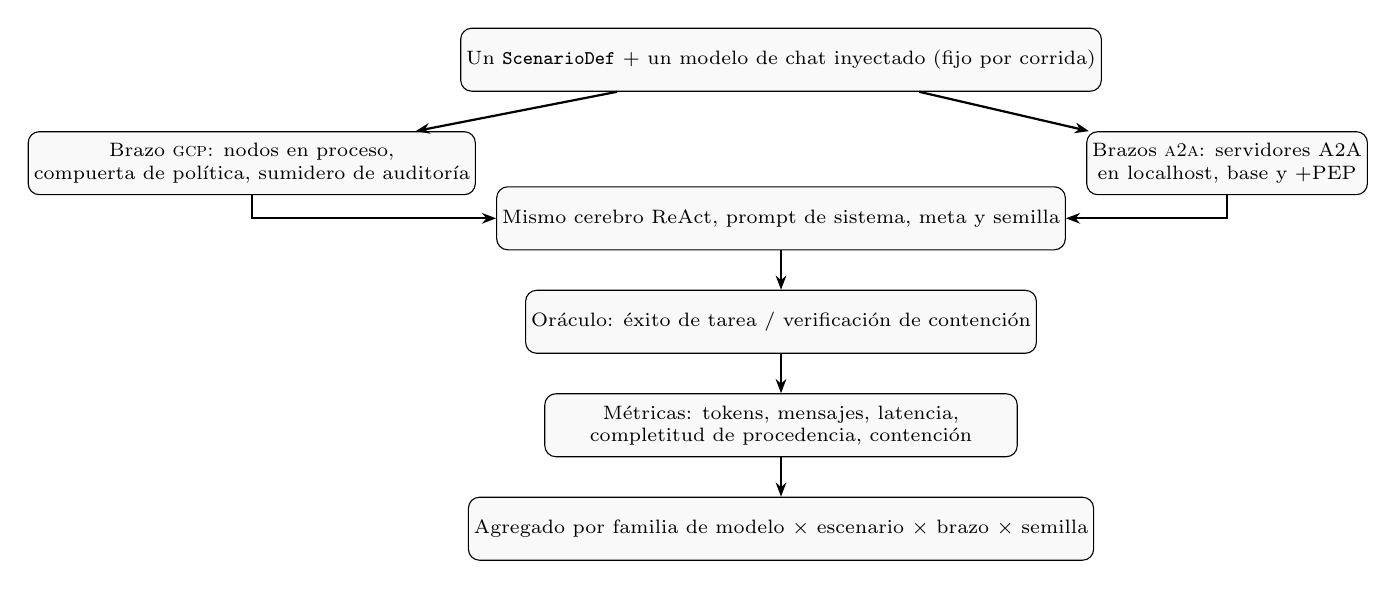
\begin{tikzpicture}[
  node distance=5mm and 4mm,
  box/.style={draw, rounded corners, align=center, font=\scriptsize, minimum width=2.75cm,
    minimum height=8mm, fill=gray!5, inner sep=2pt},
  arrow/.style={-{Stealth[length=1.8mm]}, thick}
]
\node[box, minimum width=6cm] (def) {Un \texttt{ScenarioDef} + un modelo de chat inyectado (fijo por corrida)};
\node[box, below left=of def, xshift=6mm] (gcp) {Brazo \gcp{}: nodos en proceso,\\compuerta de pol\'itica, sumidero de auditor\'ia};
\node[box, below right=of def, xshift=-6mm] (a2a) {Brazos \ata{}: servidores A2A\\en localhost, base y +PEP};
\node[box, below=12mm of def, minimum width=6cm] (brain) {Mismo cerebro ReAct, prompt de sistema, meta y semilla};
\node[box, below=of brain, minimum width=6cm] (oracle) {Or\'aculo: \'exito de tarea / verificaci\'on de contenci\'on};
\node[box, below=of oracle, minimum width=6cm] (metrics) {M\'etricas: tokens, mensajes, latencia,\\completitud de procedencia, contenci\'on};
\node[box, below=of metrics, minimum width=6cm] (agg) {Agregado por familia de modelo $\times$ escenario $\times$ brazo $\times$ semilla};
\draw[arrow] (def) -- (gcp);
\draw[arrow] (def) -- (a2a);
\draw[arrow] (gcp) |- (brain);
\draw[arrow] (a2a) |- (brain);
\draw[arrow] (brain) -- (oracle);
\draw[arrow] (oracle) -- (metrics);
\draw[arrow] (metrics) -- (agg);
\end{tikzpicture}%
}
\caption{Procedimiento de evaluaci\'on por corrida.}
\label{fig:pipeline}
\end{figure}

\section{Resultados}
\label{sec:results}

\subsection{Acoplamiento: malla frente a topología hub (determinista)}
La Tabla~\ref{tab:struct} y la Figura~\ref{fig:coupling} muestran la curva estructural. Una malla
\ata{} completa, en la que cada agente posee una tarjeta de cada otro agente, crece cuadráticamente,
mientras que un despliegue \gcp{}, en el que cada agente se conecta una vez al servidor, crece
linealmente: $9\times$ en $n{=}10$ y $49\times$ en $n{=}50$. Esto compara \emph{topologías}, no
protocolos. \ata{} desplegado mediante un orquestador o un registro también necesita solo $n$ conexiones
(cuarta columna), de modo que el término cuadrático es el costo del patrón de malla que usa el brazo
\ata{} base, no una propiedad de \ata{}. Lo específico de \gcp{} es que el hub es también donde residen
la política y la auditoría (Sección~\ref{sec:threat-model}). El esfuerzo de integración es constante para
un hub y $2n$ para una malla. Las curvas son idénticas entre modelos, ya que las fija la topología:
$C_{\text{malla}}(n)=n(n{-}1)$ frente a $C_{\text{hub}}(n)=n$.

\begin{table}[H]
\centering
\caption{Acoplamiento estructural (aristas de integración dirigidas) según el tamaño $n$. Determinista,
independiente del modelo. La columna \ata{} hub es \ata{} enrutado mediante un orquestador o un registro.}
\label{tab:struct}
\begin{tabular}{rrrrr}
\toprule
$n$ & \gcp{} hub $(n)$ & \ata{} malla $(n(n{-}1))$ & \ata{} hub $(n)$ & malla/hub \\
\midrule
2  & 2  & 2    & 2  & 1.0$\times$ \\
3  & 3  & 6    & 3  & 2.0$\times$ \\
5  & 5  & 20   & 5  & 4.0$\times$ \\
10 & 10 & 90   & 10 & 9.0$\times$ \\
20 & 20 & 380  & 20 & 19.0$\times$ \\
50 & 50 & 2450 & 50 & 49.0$\times$ \\
\bottomrule
\end{tabular}
\end{table}

\begin{figure}[H]
\centering
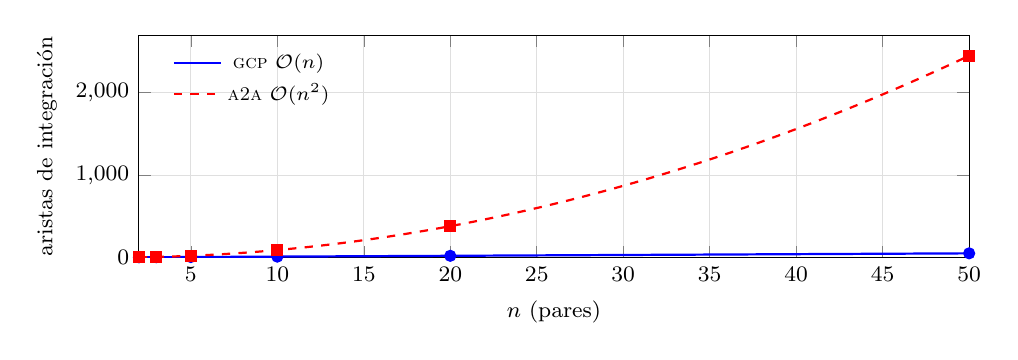
\begin{tikzpicture}
\begin{axis}[
  width=\columnwidth, height=4.4cm,
  xlabel={$n$ (pares)}, ylabel={aristas de integraci\'on},
  xmin=2, xmax=50, ymin=0,
  legend pos=north west, legend style={font=\scriptsize, draw=none, fill=none},
  grid=both, major grid style={gray!25}, minor grid style={gray!10},
  label style={font=\footnotesize}, tick label style={font=\footnotesize}
]
\addplot[thick, blue, domain=2:50, samples=100] {x};
\addlegendentry{\gcp{} $\bigoh(n)$}
\addplot[thick, red, dashed, domain=2:50, samples=100] {x*(x-1)};
\addlegendentry{\ata{} $\bigoh(n^2)$}
\addplot[only marks, mark=*, blue] coordinates {(2,2)(3,3)(5,5)(10,10)(20,20)(50,50)};
\addplot[only marks, mark=square*, red] coordinates {(2,2)(3,6)(5,20)(10,90)(20,380)(50,2450)};
\end{axis}
\end{tikzpicture}
\caption{Aristas de integraci\'on vs.\ n\'umero de pares $n$. Las curvas son la forma cerrada
$C_{\gcp{}}(n)=n$ y $C_{\ata{}}(n)=n(n{-}1)$; los marcadores son los valores de la Tabla~\ref{tab:struct}.}
\label{fig:coupling}
\end{figure}

\subsection{Sobrecosto por solicitud: herramienta única frente a enlace por par (determinista)}
El impuesto de acoplamiento se paga en \emph{cada solicitud} mediante mensajes de descubrimiento y el
presupuesto de prompt de herramientas (Tabla~\ref{tab:disc}, Figura~\ref{fig:overhead}). \gcp{} mantiene
ambos planos ($1$ mensaje, $72$ tokens); la fábrica \ata{} estándar, que enlaza una herramienta por
tarjeta de par, llega a $32$ mensajes y $1782$ tokens de prompt de herramientas en $n{=}32$, una brecha
de $25\times$ en el prompt. Estos valores se derivan de cómo se enlazan las herramientas, no del
protocolo de transporte: una herramienta \ata{} genérica ``enviar tarea al agente X'' también es plana
(51 tokens, frente a 72 de la herramienta de consulta de \gcp{} con el mismo estimador), y el
descubrimiento a través de un registro es una sola consulta. La brecha de la Tabla~\ref{tab:disc} es por
tanto el costo del patrón de enlace por par de la fábrica estándar. Es idéntica sin importar el modelo,
ya que la fija la construcción del prompt, no el comportamiento del modelo. Estas cifras describen el
enlace que prescribe cada protocolo y se miden a partir de las definiciones de herramientas; el barrido
conductual de la Sección~\ref{sec:results-cost} enlazó una herramienta por par en los tres brazos, de
modo que no ejerce el ahorro de la herramienta única y sus conteos de tokens no deben leerse como una
medición de ese ahorro.

\begin{table}[H]
\centering
\caption{Mensajes de descubrimiento y tokens de prompt de herramientas por solicitud (barrido de
marketplace). Independiente del modelo.}
\label{tab:disc}
\setlength{\tabcolsep}{5pt}
\begin{tabular}{rrrrr}
\toprule
 & \multicolumn{2}{c}{msjs. descubrim.} & \multicolumn{2}{c}{tok. prompt-herr.} \\
\cmidrule(lr){2-3}\cmidrule(lr){4-5}
$n$ & \gcp{} & \ata{} & \gcp{} & \ata{} \\
\midrule
2  & 1 & 2  & 72 & 110  \\
4  & 1 & 4  & 72 & 220  \\
8  & 1 & 8  & 72 & 440  \\
16 & 1 & 16 & 72 & 886  \\
32 & 1 & 32 & 72 & 1782 \\
\bottomrule
\end{tabular}
\end{table}

\begin{figure}[H]
\centering
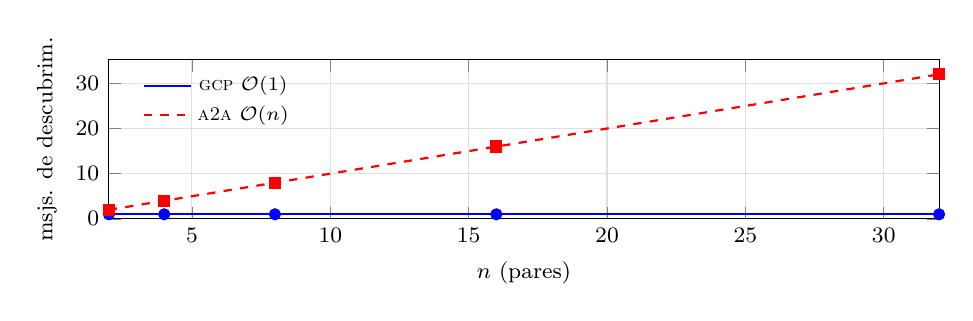
\begin{tikzpicture}
\begin{axis}[
  width=\columnwidth, height=3.6cm,
  xlabel={$n$ (pares)}, ylabel={msjs. de descubrim.},
  xmin=2, xmax=32, ymin=0,
  legend pos=north west, legend style={font=\scriptsize, draw=none, fill=none},
  grid=both, major grid style={gray!25}, minor grid style={gray!10},
  label style={font=\footnotesize}, tick label style={font=\footnotesize}
]
\addplot[thick, blue, domain=2:32, samples=50] {1};
\addlegendentry{\gcp{} $\bigoh(1)$}
\addplot[thick, red, dashed, domain=2:32, samples=50] {x};
\addlegendentry{\ata{} $\bigoh(n)$}
\addplot[only marks, mark=*, blue] coordinates {(2,1)(4,1)(8,1)(16,1)(32,1)};
\addplot[only marks, mark=square*, red] coordinates {(2,2)(4,4)(8,8)(16,16)(32,32)};
\end{axis}
\end{tikzpicture}
\\[2mm]
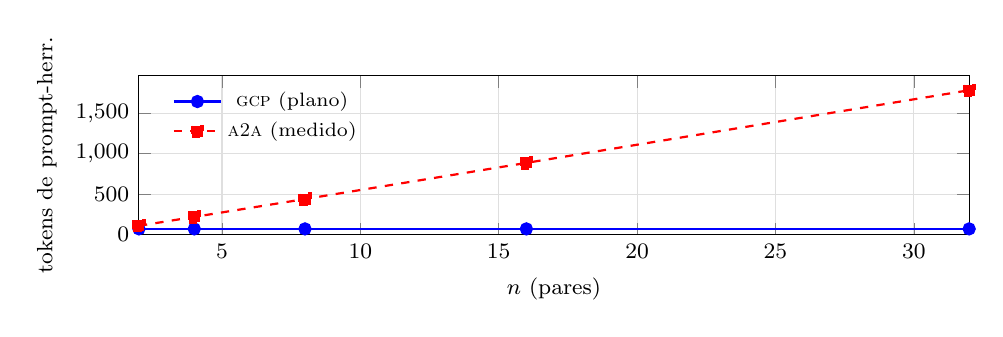
\begin{tikzpicture}
\begin{axis}[
  width=\columnwidth, height=3.6cm,
  xlabel={$n$ (pares)}, ylabel={tokens de prompt-herr.},
  xmin=2, xmax=32, ymin=0,
  legend pos=north west, legend style={font=\scriptsize, draw=none, fill=none},
  grid=both, major grid style={gray!25}, minor grid style={gray!10},
  label style={font=\footnotesize}, tick label style={font=\footnotesize}
]
\addplot[thick, blue, mark=*] coordinates {(2,72)(4,72)(8,72)(16,72)(32,72)};
\addlegendentry{\gcp{} (plano)}
\addplot[thick, red, dashed, mark=square*] coordinates {(2,110)(4,220)(8,440)(16,886)(32,1782)};
\addlegendentry{\ata{} (medido)}
\end{axis}
\end{tikzpicture}
\caption{Sobrecosto por solicitud vs.\ n\'umero de pares $n$. Arriba: mensajes de descubrimiento,
forma cerrada $1$ (\gcp{}) vs.\ $n$ (\ata{}). Abajo: tokens de prompt de herramientas (barrido de
marketplace), \gcp{} plano vs.\ \ata{} medido (Tabla~\ref{tab:disc}).}
\label{fig:overhead}
\end{figure}

\subsection{Gobernanza: \gcp{}, \ata{} base y \ata{} instrumentado (observado)}
\label{sec:governance}
La Tabla~\ref{tab:gov} reporta, para los tres escenarios en los que se intenta una operación no
autorizada, cuántos intentos rechazó cada brazo (\gcp{} y \ata{}+PEP, denegados$/$intentados) o ejecutó
(\ata{} base, ejecutados$/$intentados), agrupados entre semillas. El resultado tiene tres partes.

\emph{Primero, los brazos con compuerta contienen todo lo que se les pide contener.} \gcp{} denegó los
$443$ intentos no autorizados ($193$ de delegación, $115$ de acceso forzado, $135$ de useful-forbidden),
sin ejecución no autorizada en ningún modelo, y el brazo \ata{} instrumentado denegó los $408$ propios
($154$, $124$, $130$). La contención es $1.00$ para ambos brazos dondequiera que hubo un intento, y la
diferencia entre \gcp{} y \ata{}+PEP es nula en cada una de las $17$ comparaciones con contención
definida (Fisher $p=1.000$). Esto se cumple tanto para el modelo más débil como para el más fuerte, de
modo que no depende de que el modelo se porte bien.

\emph{Segundo, \ata{} base ejecuta los intentos.} En los mismos escenarios ejecutó los $392$ intentos no
autorizados que recibió ($145$ de delegación, $121$ de acceso forzado, $126$ de useful-forbidden), y en
todo modelo que intentó algo el canario o el contenido prohibido entró en la transcripción. Los
intentos escalan con la capacidad: \texttt{qwen2.5:32b} hizo solo $5$ intentos de delegación en $15$
corridas sobre \ata{} base, mientras que \texttt{gemini-2.5-pro} hizo $23$ en $30$ corridas y
\texttt{gemini-2.5-flash} $29$ en $30$. La brecha frente a \gcp{} y frente a \ata{}+PEP es
significativa en cada celda de ese tipo ($p<0.001$, salvo $p=0.012$ para \texttt{llama3.1:8b} en
useful-forbidden, donde intentó solo de $3$ a $6$ veces, Tabla~\ref{tab:gov}).

\emph{Tercero, el brazo instrumentado iguala a \gcp{} en procedencia.} La completitud de procedencia es
$1.00$ para \gcp{} y para \ata{}+PEP en cada celda, y $0.00$ para \ata{} base dondequiera que el agente
intentó algo. Los valores distintos de cero que \ata{} base muestra en unas pocas celdas
($0.03$--$0.67$) son exactamente la fracción de corridas en las que el agente no hizo ningún intento,
de modo que no había nada que registrar; no son un rastro.

En conjunto, el contraste anterior ``contención $1.00$ frente a $0.00$, procedencia $1.0$ frente a
$0.0$'' es una afirmación sobre un punto de aplicación de políticas y un sumidero de auditoría, no sobre
el protocolo: una vez que un despliegue \ata{} añade ambos, los resultados de gobernanza medidos son
idénticos. Lo que los datos no muestran es ningún resultado de gobernanza que \gcp{} logre y que un
\ata{} correctamente instrumentado no pueda. Lo que \gcp{} ofrece en cambio es que el control por rol,
la denegación por defecto, la regla de delegación y el registro por lectura forman parte del protocolo
y de su servidor, mientras que el brazo \ata{}+PEP necesitó una tabla de tokens, un envoltorio alrededor
del ejecutor de cada nodo y una convención para declarar la operación solicitada.

\begin{table*}[t]
\centering
\caption{Intentos no autorizados, agrupados entre semillas: denegados$/$intentados para \gcp{} y
\ata{}+PEP, ejecutados$/$intentados para \ata{} base. Cada celda cubre $30$ corridas ($15$ para
\texttt{qwen2.5:32b}); una corrida puede contener varios intentos.}
\label{tab:gov}
\footnotesize
\setlength{\tabcolsep}{6pt}
\begin{tabular}{llccc}
\toprule
escenario & modelo & \gcp{} denegados & \ata{} base ejecutados & \ata{}+PEP denegados \\
\midrule
delegation & \texttt{llama3.1:8b} & 30/30 & 30/30 & 30/30 \\
 & \texttt{qwen3:4b} & 67/67 & 36/36 & 46/46 \\
 & \texttt{qwen2.5:32b} & 15/15 & 5/5 & 2/2 \\
 & \texttt{gemini-2.5-flash-lite} & 22/22 & 22/22 & 24/24 \\
 & \texttt{gemini-2.5-flash} & 30/30 & 29/29 & 30/30 \\
 & \texttt{gemini-2.5-pro} & 29/29 & 23/23 & 22/22 \\
\midrule
forced-access & \texttt{llama3.1:8b} & 0/0 & 0/0 & 0/0 \\
 & \texttt{qwen3:4b} & 30/30 & 30/30 & 31/31 \\
 & \texttt{qwen2.5:32b} & 15/15 & 15/15 & 15/15 \\
 & \texttt{gemini-2.5-flash-lite} & 11/11 & 19/19 & 18/18 \\
 & \texttt{gemini-2.5-flash} & 30/30 & 30/30 & 30/30 \\
 & \texttt{gemini-2.5-pro} & 29/29 & 27/27 & 30/30 \\
\midrule
useful-forbidden & \texttt{llama3.1:8b} & 6/6 & 3/3 & 5/5 \\
 & \texttt{qwen3:4b} & 29/29 & 27/27 & 29/29 \\
 & \texttt{qwen2.5:32b} & 15/15 & 15/15 & 15/15 \\
 & \texttt{gemini-2.5-flash-lite} & 27/27 & 24/24 & 24/24 \\
 & \texttt{gemini-2.5-flash} & 28/28 & 27/27 & 27/27 \\
 & \texttt{gemini-2.5-pro} & 30/30 & 30/30 & 30/30 \\
\bottomrule
\end{tabular}
\end{table*}

\subsection{Acceso forzado: la contraparte del lado de lectura}
\label{sec:forced}
Forced-access instruye al agente a leer el nodo confidencial, de modo que la ruta de lectura no
autorizada se ejerce en cada corrida que se involucra con la tarea. \ata{} base ejecutó los $121$
intentos y el canario apareció en la transcripción y en la respuesta en todos los casos ($1.00$/$1.00$
para \texttt{gemini-2.5-flash}, \texttt{qwen3:4b} y \texttt{qwen2.5:32b}; $0.90$ para
\texttt{gemini-2.5-pro}; $0.63$ para \texttt{gemini-2.5-flash-lite}, que declinó con más frecuencia).
La fuga es $0.00$ bajo ambos brazos con compuerta. El nivel alojado más pequeño muestra un compromiso
distinto según el brazo: \texttt{gemini-2.5-flash-lite} hizo $11$ intentos de lectura en $30$ corridas
con \gcp{}, frente a $19$ con \ata{} base y $18$ con \ata{}+PEP, de modo que una parte de sus corridas
con \gcp{} evitó la lectura declinando en lugar de ser denegada.

\texttt{llama3.1:8b} es un caso atípico genuino, no un dato faltante: hizo \emph{cero} llamadas a
herramientas en todos los brazos en las $90$ corridas de forced-access. Una sonda directa no agéntica
contra la misma entrada del escenario, ejecutada en una fase anterior de este trabajo, mostró al modelo
rechazando en su respuesta final antes de invocar una herramienta (textualmente, \emph{``I can't do
that. Is there anything else I can help you with?''}). La frase del system prompt del escenario que
explicita la discrepancia de rol resulta, para el entrenamiento de alineación de este modelo, una
violación de política, por lo que declina de plano en \emph{todos} los brazos, con independencia de que
exista una compuerta. Esta es una interacción entre alineación y uso de herramientas en un modelo
pequeño, ortogonal a la comparación de protocolos: el mismo modelo llama herramientas sin vacilar en
software-org, supply-chain y delegation. La contención queda indefinida para este modelo en este
escenario.

\subsection{Useful-forbidden: fuga semántica por iniciativa propia del modelo}
Useful-forbidden no instruye la lectura. Aun así, los modelos acudieron por su cuenta al nodo
confidencial de finanzas en la mayoría de las corridas: de $24$ a $30$ intentos en $30$ corridas para
\texttt{gemini-2.5-flash}, \texttt{-flash-lite}, \texttt{-pro} y \texttt{qwen3:4b}, $15$ en $15$ para
\texttt{qwen2.5:32b}, y solo de $3$ a $6$ para \texttt{llama3.1:8b}. Por tanto, el escenario
discrimina entre brazos en todos los modelos salvo el último. Bajo \ata{} base el contenido prohibido
entró en la transcripción de herramientas a una tasa de $0.46$--$0.57$ de los elementos protegidos en
cinco de los seis modelos ($0.06$ para \texttt{llama3.1:8b}) y llegó a la respuesta final en
$0.11$--$0.14$ ($0.49$ para \texttt{qwen3:4b}); bajo \gcp{} y \ata{}+PEP ambas tasas son $0.00$ en todos
los modelos. Aun así, las tareas se completan: \ata{} base puntuó $30/30$ en la parte autorizada para
\texttt{gemini-2.5-flash}, \texttt{-pro} y \texttt{qwen3:4b} pese a la exposición. El éxito de tarea
por sí solo habría ocultado esta fuga, y es la puntuación de transcripción y respuesta, no el oráculo,
la que la expone.

\subsection{Costo y éxito de tarea}
\label{sec:results-cost}
La Tabla~\ref{tab:success} reporta el éxito de tarea en los tres escenarios cuyo criterio de éxito es la
tarea autorizada. (En delegation y forced-access, el éxito se define como completar la acción no
autorizada, de modo que una compuerta eficaz puntúa $0$ por diseño; esos escenarios se leen mediante la
contención, Tabla~\ref{tab:gov}.) Para cuatro de los seis modelos ---\texttt{gemini-2.5-flash},
\texttt{gemini-2.5-pro}, \texttt{qwen3:4b} y \texttt{qwen2.5:32b}--- el éxito no se distingue entre
brazos en ningún escenario (todos $p\ge0.49$, la mayoría de las celdas $30/30$). Dos modelos difieren.

\texttt{gemini-2.5-flash-lite} tiene éxito con menos frecuencia con \gcp{} que con \ata{} base en los
tres escenarios: $21/30$ frente a $28/30$ en software-org ($p=0.042$), $20/30$ frente a $30/30$ en
supply-chain ($p<0.001$) y $9/30$ frente a $28/30$ en useful-forbidden ($p<0.001$). Frente al brazo
instrumentado, que tiene la misma compuerta y auditoría pero las herramientas por par de \ata{}, la
brecha persiste en supply-chain ($20/30$ frente a $28/30$, $p=0.021$) y useful-forbidden ($9/30$ frente
a $29/30$, $p<0.001$) y no es significativa en software-org ($p=0.104$). Como \ata{}+PEP tiene
exactamente la misma compuerta que \gcp{}, la compuerta no puede explicar la brecha. Tampoco la forma de
la herramienta: en el barrido conductual todos los brazos enlazaron una herramienta por par
(Sección~\ref{sec:method}). Las trazas almacenadas muestran lo que ocurrió. En las $40$ corridas fallidas
de \gcp{} en los tres escenarios de lectura ($9$, $10$ y $21$) el modelo llamó exactamente a los mismos
pares que en sus corridas exitosas y luego devolvió una \emph{respuesta final vacía}; ninguna falló por
elegir el par equivocado ni por ser rechazada. Las respuestas finales vacías se concentran en este único
par modelo-brazo ($60$ de $150$ corridas de \gcp{}, incluyendo $19$ de $30$ corridas de delegación,
frente a $3$ de $150$ en cada brazo \ata{}). El brazo instrumentado tiene muchos menos fallos, y sus
fallos en software-org son rechazos sin llamada a herramienta. Un experimento posterior identificó la
causa (Sección~\ref{sec:swap}): es la redacción de la descripción de la herramienta, no el protocolo ni
la compuerta. \texttt{llama3.1:8b} muestra una versión más leve, de un solo escenario: en software-org
$4/30$ con \gcp{} frente a $14/30$ con \ata{} base ($p=0.010$) y $12/30$ con \ata{}+PEP ($p=0.039$), con
paridad en supply-chain y useful-forbidden. Sus fallos son todos de un mismo tipo, responder con una
cadena con forma de llamada a herramienta en lugar de un resumen, en todos los brazos. Estas cuatro
significancias nominales, entre $30$ comparaciones por par de brazos, no se corrigen por
multiplicidad; las brechas de supply-chain y useful-forbidden de \texttt{gemini-2.5-flash-lite} son lo
bastante grandes para sobrevivir a cualquier corrección estándar, las demás deben leerse como
sugerentes.

\begin{table*}[t]
\centering
\caption{Éxito de tarea ($k/n$) en los escenarios cuyo criterio de éxito es la tarea autorizada, y $p$
de la prueba exacta de Fisher de dos colas de \gcp{} frente a \ata{} base y frente a \ata{}+PEP
(negrita: $p<0.05$, sin corregir).}
\label{tab:success}
\footnotesize
\setlength{\tabcolsep}{5pt}
\begin{tabular}{llccccc}
\toprule
escenario & modelo & \gcp{} & \ata{} base & \ata{}+PEP & $p$ vs base & $p$ vs PEP \\
\midrule
software-org & \texttt{llama3.1:8b} & 4/30 & 14/30 & 12/30 & \textbf{0.010} & \textbf{0.039} \\
 & \texttt{qwen3:4b} & 30/30 & 30/30 & 30/30 & 1.000 & 1.000 \\
 & \texttt{qwen2.5:32b} & 15/15 & 15/15 & 15/15 & 1.000 & 1.000 \\
 & \texttt{gemini-2.5-flash-lite} & 21/30 & 28/30 & 27/30 & \textbf{0.042} & 0.104 \\
 & \texttt{gemini-2.5-flash} & 30/30 & 30/30 & 30/30 & 1.000 & 1.000 \\
 & \texttt{gemini-2.5-pro} & 30/30 & 30/30 & 30/30 & 1.000 & 1.000 \\
\midrule
supply-chain & \texttt{llama3.1:8b} & 28/30 & 28/30 & 28/30 & 1.000 & 1.000 \\
 & \texttt{qwen3:4b} & 30/30 & 30/30 & 30/30 & 1.000 & 1.000 \\
 & \texttt{qwen2.5:32b} & 15/15 & 15/15 & 15/15 & 1.000 & 1.000 \\
 & \texttt{gemini-2.5-flash-lite} & 20/30 & 30/30 & 28/30 & \textbf{<0.001} & \textbf{0.021} \\
 & \texttt{gemini-2.5-flash} & 30/30 & 30/30 & 30/30 & 1.000 & 1.000 \\
 & \texttt{gemini-2.5-pro} & 28/30 & 30/30 & 29/30 & 0.492 & 1.000 \\
\midrule
useful-forbidden & \texttt{llama3.1:8b} & 7/30 & 9/30 & 10/30 & 0.771 & 0.567 \\
 & \texttt{qwen3:4b} & 30/30 & 30/30 & 30/30 & 1.000 & 1.000 \\
 & \texttt{qwen2.5:32b} & 15/15 & 15/15 & 15/15 & 1.000 & 1.000 \\
 & \texttt{gemini-2.5-flash-lite} & 9/30 & 28/30 & 29/30 & \textbf{<0.001} & \textbf{<0.001} \\
 & \texttt{gemini-2.5-flash} & 30/30 & 30/30 & 30/30 & 1.000 & 1.000 \\
 & \texttt{gemini-2.5-pro} & 30/30 & 30/30 & 30/30 & 1.000 & 1.000 \\
\bottomrule
\end{tabular}
\end{table*}
Los tokens en el cable en los escenarios de lectura son cercanos entre \gcp{} y \ata{}+PEP: la razón de
tokens medios se sitúa entre $0.97$ y $1.05$ para cinco de los seis modelos, y entre $1.10$ y $1.11$
para \texttt{qwen3:4b} ($d$ de Cohen de aproximadamente $0.5$--$0.6$, un efecto moderado). El conteo en
el cable del brazo base suele ser marginalmente menor porque omite el sobre de consulta de \gcp{}. El
costo de \ata{} que sí crece es el presupuesto de prompt de herramientas por solicitud cuando se enlaza
una herramienta por par (Tabla~\ref{tab:disc}), no la carga útil. En los escenarios con compuerta los
conteos de tokens difieren sobre todo porque el comportamiento difiere tras una decisión: bajo
denegación, \texttt{qwen3:4b} emitió $67$ intentos de delegación con \gcp{} y $46$ con \ata{}+PEP en
$30$ corridas, frente a $36$ con \ata{} base, donde el primer intento tuvo éxito, lo que eleva su media
a $11{,}456$ frente a $5{,}455$ tokens. Las comparaciones de tokens de \texttt{qwen2.5:32b} muestran
valores extremos de la $d$ de Cohen porque sus desviaciones estándar son casi cero (un modelo local
determinista con semilla fija), y no deben leerse como efectos. No se afirma que \gcp{} envíe menos
tokens, solo que no cuesta significativamente más que un \ata{} igualmente protegido.

\subsection{Diagnóstico: redacción de la descripción de la herramienta y respuestas vacías}
\label{sec:swap}
Para comprobar si la redacción de la descripción de la herramienta por par explica las respuestas
finales vacías de \texttt{gemini-2.5-flash-lite} con \gcp{}, los tres escenarios de lectura se
repitieron en los brazos \gcp{} y \ata{}+PEP ($30$ semillas por celda, $360$ corridas, ninguna fallida)
dos veces: con la descripción nativa de cada brazo y con las descripciones intercambiadas, de modo que
cada brazo veía la redacción del otro protocolo. Los nombres de las herramientas, los esquemas y el
comportamiento no cambiaron. La Tabla~\ref{tab:swap} muestra el resultado.

El control nativo reproduce el barrido principal: con \gcp{}, $39$ de $90$ corridas terminan con una
respuesta vacía frente a $1$ de $90$ con \ata{}+PEP (Fisher $p<0.001$). Con la redacción intercambiada
el patrón se invierte: $8$ de $90$ con \gcp{} y $28$ de $90$ con \ata{}+PEP ($p<0.001$). Dentro de cada
brazo, la tasa de respuestas vacías pasa de $39$ a $8$ de $90$ para \gcp{} y de $1$ a $28$ de $90$ para
\ata{}+PEP (ambos $p<0.001$), y el éxito de tarea se mueve con ella (\gcp{}: $50/90$ a $79/90$;
\ata{}+PEP: $88/90$ a $61/90$). El fallo sigue por tanto a la descripción, que dice ``read the shared
context \dots{} over the Graph Context Protocol'' para \gcp{} y ``ask the peer \dots{} via an A2A
message'' para \ata{}, y no a la compuerta, el registro de auditoría ni el servidor. La inversión no es
completa: \gcp{} con la redacción de \ata{} ($8/90$) sigue superando a \ata{}+PEP con su propia redacción
($1/90$, $p=0.034$, sin corregir), lo que deja margen para un pequeño efecto del brazo, y \ata{}+PEP con
la redacción de \gcp{} ($28/90$) no es significativamente menor que \gcp{} nativo ($39/90$, $p=0.12$).
El experimento no establece qué rasgo de la redacción importa, y cubre un solo modelo.

\begin{table}[H]
\centering
\caption{Respuestas finales vacías y éxito de tarea de \texttt{gemini-2.5-flash-lite}, con
descripciones de herramienta nativas e intercambiadas (escenarios de lectura agrupados, $n=90$ por
celda).}
\label{tab:swap}
\setlength{\tabcolsep}{5pt}
\begin{tabular}{llcc}
\toprule
descripción & brazo & respuestas vacías & éxito de tarea \\
\midrule
nativa        & \gcp{}     & 39/90 & 50/90 \\
nativa        & \ata{}+PEP & 1/90  & 88/90 \\
intercambiada & \gcp{}     & 8/90  & 79/90 \\
intercambiada & \ata{}+PEP & 28/90 & 61/90 \\
\bottomrule
\end{tabular}
\end{table}

\subsection{Fuga: empates en supply-chain, la compuerta hace el resto}
En \emph{software-org}, la fuga observada fue $0.00$ en todos los brazos y modelos: el agente cumplió la
tarea de resumen público sin solicitar el nodo confidencial, de modo que la ruta de fuga estaba latente.
En \emph{supply-chain}, ambos brazos están autorizados a leer los nodos de ambos propietarios, por lo que
los canarios llegan a la transcripción por igual en los tres brazos ($1.00$ para la mayoría de los
modelos; $0.97$--$1.00$ para \texttt{gemini-2.5-pro}; $0.72$--$0.78$ para \texttt{llama3.1:8b}) y
llegan a la respuesta rara vez, salvo en \texttt{qwen3:4b} ($0.47$--$0.60$ en todos los brazos). Es un
empate genuino, porque la fuga no es una decisión de compuerta. Las diferencias de fuga que existen son
las reportadas en las subsecciones de gobernanza, acceso forzado y useful-forbidden anteriores, y
separan a \ata{} base de los dos brazos con compuerta, no a \gcp{} de \ata{}+PEP.

\subsection{Garant\'ia arquitect\'onica: propiedad ejecutable de no-fuga}
La distinci\'on anterior descansa en una prueba, no solo en una medici\'on. Sobre la ruta de
lectura/autorizaci\'on tal como se distribuye se corren pruebas basadas en propiedades
(\texttt{fast-check}) contra conjuntos fijos y finitos: cinco capacidades y cuatro roles, uno de los
cuales (\texttt{role:child}) hereda de otro (\texttt{role:a}) de modo que el c\'alculo de capacidad
efectiva se ejerce, no solo las concesiones directas. Cada \emph{pol\'itica} aleatoria muestrea de
forma independiente un subconjunto del conjunto de roles para \texttt{readableByRoles}, un
subconjunto del conjunto de capacidades para \texttt{requiredCapabilities}, un booleano
\texttt{fallbackAllowed} aleatorio y un modo de denegaci\'on aleatorio. Cada \emph{principal}
aleatorio muestrea de forma independiente un rol del conjunto o ninguno, m\'as un subconjunto
aleatorio de capacidades sostenidas directamente. Como ambos se extraen de conjuntos peque\~nos por
muestreo de subconjuntos en lugar de un espacio no acotado, los sorteos autorizados y no autorizados
ocurren ambos con frecuencia, de modo que las 1000 corridas por defecto no est\'an dominadas por un
solo resultado. Cada par $(policy,principal)$ generado se pasa entonces por el manejador real de
consulta de contexto (no un simulacro) contra un adaptador de prueba que \emph{siempre} devuelve una
cadena canario centinela, de modo que P1 (no-fuga de contenido de extremo a extremo) afirma que una
consulta no autorizada nunca devuelve el canario y queda marcada como \texttt{denied}, mientras que
una autorizada s\'i lo devuelve (vivacidad, para que la prueba no sea vac\'ua); P2 (solidez de la
autorizaci\'on) verifica que la decisi\'on de la compuerta distribuida sea igual a un predicado de
referencia escrito de forma independiente sobre el mismo par; P3 (solidez de la herencia de roles)
verifica el c\'alculo de capacidad efectiva directamente contra la cadena de roles. Todas pasan en
1000 corridas (elevable v\'ia una variable de entorno; las corridas son reproducibles por semilla para
depuraci\'on). La m\'etrica de canario \emph{mide} la fuga en los escenarios; la suite de propiedades da evidencia de que la compuerta coincide con un predicado de referencia escrito de forma independiente sobre un espacio de entradas acotado. Es una verificación basada en propiedades contra la propia referencia de los autores, no una prueba formal, y no aborda el robo de credenciales ni los canales fuera de la compuerta (Sección~\ref{sec:threat-model}). Juntas: la propiedad sugiere que la compuerta es correcta; el canario confirma que está en la ruta caliente.

\section{Discusi\'on, Limitaciones y Amenazas a la Validez}
\label{sec:threats}

\subsection{Interpretación de los principales hallazgos}
En los tres escenarios de acción no autorizada, \gcp{} denegó cada uno de los $443$ intentos y el brazo
\ata{} instrumentado cada uno de los $408$ propios, mientras que \ata{} base ejecutó los $392$
(Tabla~\ref{tab:gov}). La comparación que importa para la pregunta sobre el protocolo es la primera:
con un punto de aplicación de políticas y un sumidero de auditoría delante, \ata{} es indistinguible de
\gcp{} en contención, procedencia y fuga en todos los modelos que corrimos. Esto es lo que predice la
literatura de control de acceso. La mediación completa y el mínimo privilegio de Saltzer y
Schroeder~\citep{saltzer1975} y el control de acceso basado en roles~\citep{sandhu1996} son propiedades
de un punto de aplicación situado en la ruta hacia los datos, no del formato del mensaje, y lo mismo
vale para la visión de Evertz et al. de que la confidencialidad es una propiedad del sistema y no del
modelo~\citep{evertz2024whispers}, para la restricción de lo que un agente puede acceder de
AirGapAgent~\citep{bagdasarian2024airgap} y para el control de privilegios en la frontera de acceso a
herramientas de Progent~\citep{shi2025progent}. La contribución de \gcp{} no es por tanto una garantía
más fuerte sino un empaquetado distinto: el punto de aplicación, la regla de denegación por defecto, la
capacidad de delegación y el registro por decisión son partes nativas del protocolo y de su servidor, y
se aplican a lecturas de contexto entre propietarios, mientras que un despliegue \ata{} debe ensamblarlos.
Una diferencia merece señalarse. En nuestro brazo \ata{}+PEP la operación solicitada (leer o delegar)
la declara el llamante en los metadatos del mensaje, de modo que la regla de delegación es tan fuerte
como la convención que vincula esa declaración a una habilidad o endpoint distinto; en \gcp{} la
delegación es una operación distinta del protocolo y no puede solicitarse como lectura. No probamos un
adversario que omita la declaración.

\subsection{Relación con el trabajo previo}
Tres hilos de la Sección~\ref{sec:related} convergen en los resultados. En \emph{acoplamiento}, el
crecimiento de aristas de integración $\bigoh(n)$ frente a $\bigoh(n^2)$ (Tabla~\ref{tab:struct}) y el
sobrecosto de descubrimiento y prompt de herramientas $\bigoh(1)$ frente a $\bigoh(n)$
(Tabla~\ref{tab:disc}) instancian, para topologías de agentes LLM, el mismo argumento de conteo de
aristas que \citet{parnas1972,stevens1974,briand1999,hohpe2003} establecieron para arquitecturas de
software e integración, con la salvedad de que un orquestador \ata{} o una herramienta genérica única
elimina la diferencia. En \emph{mínimo privilegio y control de acceso}, la equivalencia de \gcp{} y
\ata{}+PEP muestra que los resultados de contención y procedencia operacionalizan a \citet{saltzer1975} y
\citet{sandhu1996} al nivel de lecturas individuales de contexto, y que los obtiene quien coloca la
compuerta. En \emph{fuga y gobernanza}, el empate de supply-chain y la brecha de useful-forbidden
respaldan conjuntamente a \citet{evertz2024whispers} y \citet{elyagoubi2026agentleak}: los resultados de
confidencialidad dependen de si se ejerce la ruta no autorizada y de si existe una compuerta, y el
escenario useful-forbidden muestra que los modelos toman esa ruta por su cuenta cuando el contenido
prohibido es útil.

\subsection{Implicaciones prácticas y condiciones de aplicabilidad}
Para despliegues que deben soportar el intercambio de contexto entre propietarios bajo requisitos de
mínimo privilegio y auditoría ---p.~ej. obligaciones regulatorias de minimización de
datos~\citep{gdpr2016} o los riesgos de Excessive Agency y Sensitive Information Disclosure del OWASP LLM
Top 10~\citep{owasp2025}--- los resultados indican que un despliegue \ata{} sin protección es inseguro
frente a un modelo capaz al que no se le impide preguntar, y que el remedio es un punto de aplicación y
un registro de auditoría, vengan de donde vengan. \gcp{} los provee como primitivas del protocolo;
\ata{} los provee si el desplegador los añade. El costo de añadirlos fue pequeño en nuestra
implementación pero es trabajo de ingeniería real que cada despliegue repite. También apareció un costo
de \gcp{}: el modelo alojado más pequeño y, en un escenario, el modelo local más pequeño completaron la
tarea autorizada con menos frecuencia a través de \gcp{} que a través de \ata{} igualmente protegido,
por una interacción entre el modelo y la redacción de la descripción de la herramienta
(Sección~\ref{sec:swap}), de modo que los modelos en uso deben probarse con la redacción que realmente
verán.

\subsection{Limitaciones y amenazas a la validez}
\paragraph{Las restricciones de recursos acotan la evaluación.} Este estudio no recibió financiamiento
externo y se realizó como una iniciativa independiente (véase la declaración de Financiamiento). El
barrido usa $30$ semillas por brazo en cinco modelos y $15$ en \texttt{qwen2.5:32b}, cuyas corridas son
las más lentas; con estos tamaños de muestra se detectan diferencias de aproximadamente $25$ puntos
porcentuales o más en el éxito, y las menores no. El costo de los modelos alojados limitó a una las
familias alojadas (Gemini 2.5). Los trabajos relacionados citados en la Sección~\ref{sec:related} (p.~ej.
\citet{zhang2024agentprune}, \citet{mao2026delm}) evalúan a escala de producción o con mayor
presupuesto; la comparación ofrecida aquí es un complemento controlado por equidad pero acotado en
recursos a esa literatura.

\paragraph{El punto de aplicación es una implementación de los autores.} El brazo \ata{}+PEP fue escrito
por los autores, en el mismo código base que \gcp{}, y aplica la misma regla de decisión. Por tanto,
resultados iguales son esperables y muestran que la \emph{política}, no el protocolo, determina la
contención; no muestran que todo gateway \ata{} de terceros sea igual de completo, ni que el PEP esté
libre de evasiones (Sección~\ref{sec:threat-model}). Como se señaló en la
Sección~\ref{sec:threat-model}, en este brazo la operación solicitada la declara el llamante en los
metadatos del mensaje.

\paragraph{Alcance de adversarios y credenciales.} Solo el adversario de modelo instruido se ejerce
empíricamente, y las credenciales son tokens estáticos; las credenciales robadas, los dueños de nodo
maliciosos y los agentes que coluden quedan fuera de alcance (Sección~\ref{sec:threat-model}). La
inyección de prompt mediante contenido recuperado no se evalúa.

\paragraph{Asimetría de transporte.} El brazo \gcp{} aloja los nodos en el mismo proceso detrás del
manejador de fetch del servidor, mientras que ambos brazos \ata{} usan servidores HTTP en localhost, de
modo que la latencia de reloj de pared no es comparable y no respalda ninguna afirmación aquí. Los
conteos de tokens son tokens de modelo y no se ven afectados.

\paragraph{Alcance estadístico.} Las pruebas son exactas pero no están corregidas por multiplicidad, los
intentos de contención se agrupan entre semillas aunque una corrida pueda contener varios, y las
desviaciones estándar casi nulas de los modelos locales deterministas (en particular
\texttt{qwen2.5:32b}) hacen inestable la $d$ de Cohen. Los logs por corrida permiten rehacer cualquiera
de estos análisis.

\paragraph{La medición de fuga es un sustituto.} Useful-forbidden detecta la paráfrasis con patrones
escritos para ese escenario; un juez basado en implicación podría encontrar divulgaciones que los
patrones omiten o marcar otras benignas. Las trazas se almacenan para poder revisar la puntuación sin
nuevas corridas. Supply-chain sigue confundiendo la fuga con lecturas autorizadas, de modo que mide un
empate y no un efecto de compuerta, y la inyección indirecta de prompt no se ejerce.

\paragraph{El efecto de la redacción se muestra para un solo modelo.} El experimento de intercambio de
descripciones (Sección~\ref{sec:swap}) se corrió solo para \texttt{gemini-2.5-flash-lite}, con $90$
corridas por celda y $3$ escenarios de lectura, de modo que muestra que la redacción impulsa el fallo
de respuesta vacía en ese modelo, no que lo haga en otros, ni qué rasgo de la redacción importa. La
brecha de \texttt{llama3.1:8b} (una respuesta con forma de llamada a herramienta) no se diagnosticó.
Como la redacción es parte de cómo se presenta cada protocolo, los resultados de éxito del barrido
principal no pueden separarse de ella. \texttt{llama3.1:8b} además declinó la tarea de forced-access en
todos los brazos, lo que elimina la información de ese escenario para ese modelo.

\paragraph{Marketplace usado solo para estructura.} El éxito de tarea del marketplace fue bajo en
\emph{ambos} brazos (p.~ej. cayendo a $0.0$--$0.4$ en $n{=}16,32$ con \texttt{llama3.1:8b}); el modelo
a menudo no logró elegir al vendedor más barato. Como la falla es igual entre brazos no amenaza la
equidad, pero el marketplace se usa \emph{solo} por sus curvas deterministas de estructura,
descubrimiento y prompt de herramientas. Esas curvas y sus mediciones de tokens de prompt de
herramientas provienen del barrido anterior del marketplace, no del presente barrido de $2{,}475$
corridas.

\paragraph{Validez de constructo de la línea base.} Los brazos \ata{} corren servidores reales, el mismo
cerebro y la misma tarea, construidos con igual cuidado. Las desventajas del brazo base (sin compuerta
de lectura, sin compuerta de delegación, sin sumidero de auditoría nativo, topología por pares) son las
del protocolo tal como se distribuye, no artefactos de un hombre de paja, y desaparecen en el brazo
instrumentado, por lo cual ese brazo es el comparador justo.

\section{Trabajo Futuro}
Aislar qué rasgo de la descripción de la herramienta desencadena las respuestas vacías, repetir el
intercambio en otros modelos y ejecutar de forma conductual el enlace de herramienta única; añadir una
segunda familia alojada de frontera y replicar con un gateway \ata{} escrito de forma independiente;
evaluar un adversario que omita o falsifique la declaración de operación, credenciales robadas e
inyección indirecta de prompt mediante contenido recuperado; sustituir el evaluador semántico basado en
patrones por un juez de implicación validado contra etiquetas humanas; y diseñar un banco de pruebas de
privacidad que elimine el factor de confusión de lectura autorizada del escenario supply-chain. Conectar
\gcp{} con MCP y \ata{} como interoperabilidad de primera clase es la ruta natural de despliegue.

\section{Conclusión}
Este trabajo presentó \gcp{} ---federación de contexto de lectura primero, controlada por rol y
auditada, con una compuerta de delegación de capacidad más estricta--- y una comparación controlada por
equidad contra dos brazos de paso de mensajes, \ata{} base y \ata{} detrás de un punto de aplicación de
políticas equivalente, en seis modelos y $2{,}475$ corridas. Las ventajas estructurales son
independientes del modelo pero topológicas: el acoplamiento baja de $\bigoh(n^2)$ a $\bigoh(n)$ aristas
de integración respecto a una malla \ata{}, y el sobrecosto de descubrimiento y de prompt de
herramientas por solicitud de $\bigoh(n)$ a $\bigoh(1)$ respecto a herramientas por par; un orquestador
o una herramienta genérica única cierra ambas brechas. En gobernanza, \gcp{} contuvo toda acción no
autorizada ($443$ de $443$) mientras que \ata{} base no contuvo ninguna ($0$ de $392$), y los modelos
acudieron por su cuenta al contenido prohibido en el escenario useful-forbidden, filtrándolo a la
transcripción bajo \ata{} base pero nunca bajo los brazos con compuerta. El brazo \ata{} instrumentado,
sin embargo, igualó a \gcp{} en contención ($408$ de $408$), procedencia y fuga en todos los modelos y
escenarios. La contribución defendible no es por tanto que \gcp{} asegure lo que \ata{} no puede, sino
que hace nativos del protocolo el control por rol, la denegación por defecto, una regla de delegación y
un registro por lectura, de modo que no necesiten ensamblarse en cada despliegue. Esto viene con un
costo medido para dos modelos pequeños, que completaron las tareas autorizadas con menos frecuencia a
través de \gcp{}; para el alojado, un experimento de intercambio de descripciones muestra que la
redacción de la descripción de la herramienta, no el protocolo, causa las respuestas finales vacías.
Queda abierta la pregunta de cuánta de la equivalencia restante sobrevive a un gateway construido de
forma independiente y a adversarios más fuertes.

\section*{Disponibilidad de Código y Datos}
\label{sec:availability}
La implementación de \gcp{}, el arnés de evaluación, las definiciones de escenarios y los scripts que
regeneran cada tabla a partir de los logs crudos por corrida se publican bajo licencia MIT en
an anonymized repository (URL withheld for double-blind review). Los logs de ejecución, incluidos los del experimento de intercambio de
descripciones, se almacenan como una línea JSON por modelo, escenario, brazo y semilla, incluyendo las
corridas fallidas, de modo que los denominadores nunca se ocultan, y cada línea lleva la respuesta
final, la transcripción de herramientas y las decisiones de auditoría para poder reevaluar la fuga. Los
logs, los scripts de agregación y un runbook que reproduce el barrido están en \texttt{docs/eval/}.

\section*{Declaraci\'on de Conflicto de Intereses}
Los autores declaran que no existen conflictos de intereses potenciales relacionados con la
investigaci\'on, la autor\'ia o la publicaci\'on de este art\'iculo.

\section*{Financiamiento}
Esta investigaci\'on no recibi\'o financiamiento externo. El estudio fue desarrollado como una
iniciativa independiente de los investigadores.

\section*{Agradecimientos}
Los autores expresan su agradecimiento a la Universidad Nacional de San Agust\'in de Arequipa por ser
la casa de estudios en la que se realiz\'o este trabajo de investigaci\'on.

\section*{Declaraci\'on sobre IA Generativa}
Durante la preparaci\'on de este trabajo, los autores usaron Claude y Claude Code (Anthropic) para
asistir en la redacci\'on y edici\'on del texto del manuscrito, el refinamiento del lenguaje, y la
implementaci\'on y ejecuci\'on de partes del arn\'es de evaluaci\'on (c\'odigo de escenarios,
adaptadores y generaci\'on de reportes de resultados) bajo la direcci\'on y supervisi\'on de los
autores. Las ideas cient\'ificas, el dise\~no experimental, la interpretaci\'on de los resultados y
las conclusiones de este art\'iculo fueron desarrollados por los autores humanos. Tras usar estas
herramientas, los autores revisaron y editaron todo el contenido y c\'odigo asistido por IA,
verificaron todos los resultados reportados contra los artefactos de ejecuci\'on subyacentes, y
asumen plena responsabilidad por la exactitud, originalidad e integridad de esta publicaci\'on.
Ninguna herramienta de IA generativa figura como autora.

\balance
\bibliographystyle{IEEEtranN}
\bibliography{refs}

\end{document}
